\documentclass[]{beamer}

\usepackage{fontspec} 
% \usepackage{lsp-makros}
\useoutertheme{lsp}

\usepackage{lsptitle}

\def\two@digits#1{\ifnum#1<10 0\fi\number#1}
\def\mytoday{\two@digits{\number\day}.\two@digits{\number\month}.\number\year}


\usepackage{xspace,multicol}
\newcommand{\latex}{\LaTeX\xspace}
\usepackage{tikz}


\newcounter{lastpagemainpart}
\footnotesep0pt
\renewcommand{\footnoterule}{}
\usefootnotetemplate{
  \noindent
  \insertfootnotemark\insertfootnotetext}

\let\beamerfn=\footnote
\renewcommand{\footnote}[1]{%
\let\oldfnsize=\footnotesize%
\let\footnotesize=\tiny%
\beamerfn<\thebeamerpauses->{#1}%
\let\footnotesize=\oldfnsize}


\date{2017-11-03}

\usepackage{eurosym}  
 
\renewcommand{\centerline}[1]{\hfill#1\hfill\hfill\mbox{}}


\title{\mbox{Community-based publishing}}
\institute{Workshop FID Afrikanistik }
\author[LangSci]{Sebastian Nordhoff}



\begin{document}
\lspbeamertitle

\section{Language Science Press}
\frame{
\frametitle{Language Science Press}
%   \includegraphics[height=.2\textheight]{./path/to/graphicsfile}
  \begin{itemize}
    \item linguistische Monographien und Sammelbände als CC-BY
    \item  aktiv seit 2014 (FU Berlin), seit 2017 HU Berlin
    \item  20 Reihen,  160 Herausgeber weltweit     
  \end{itemize}
  
%   \hspace*{-1cm}
  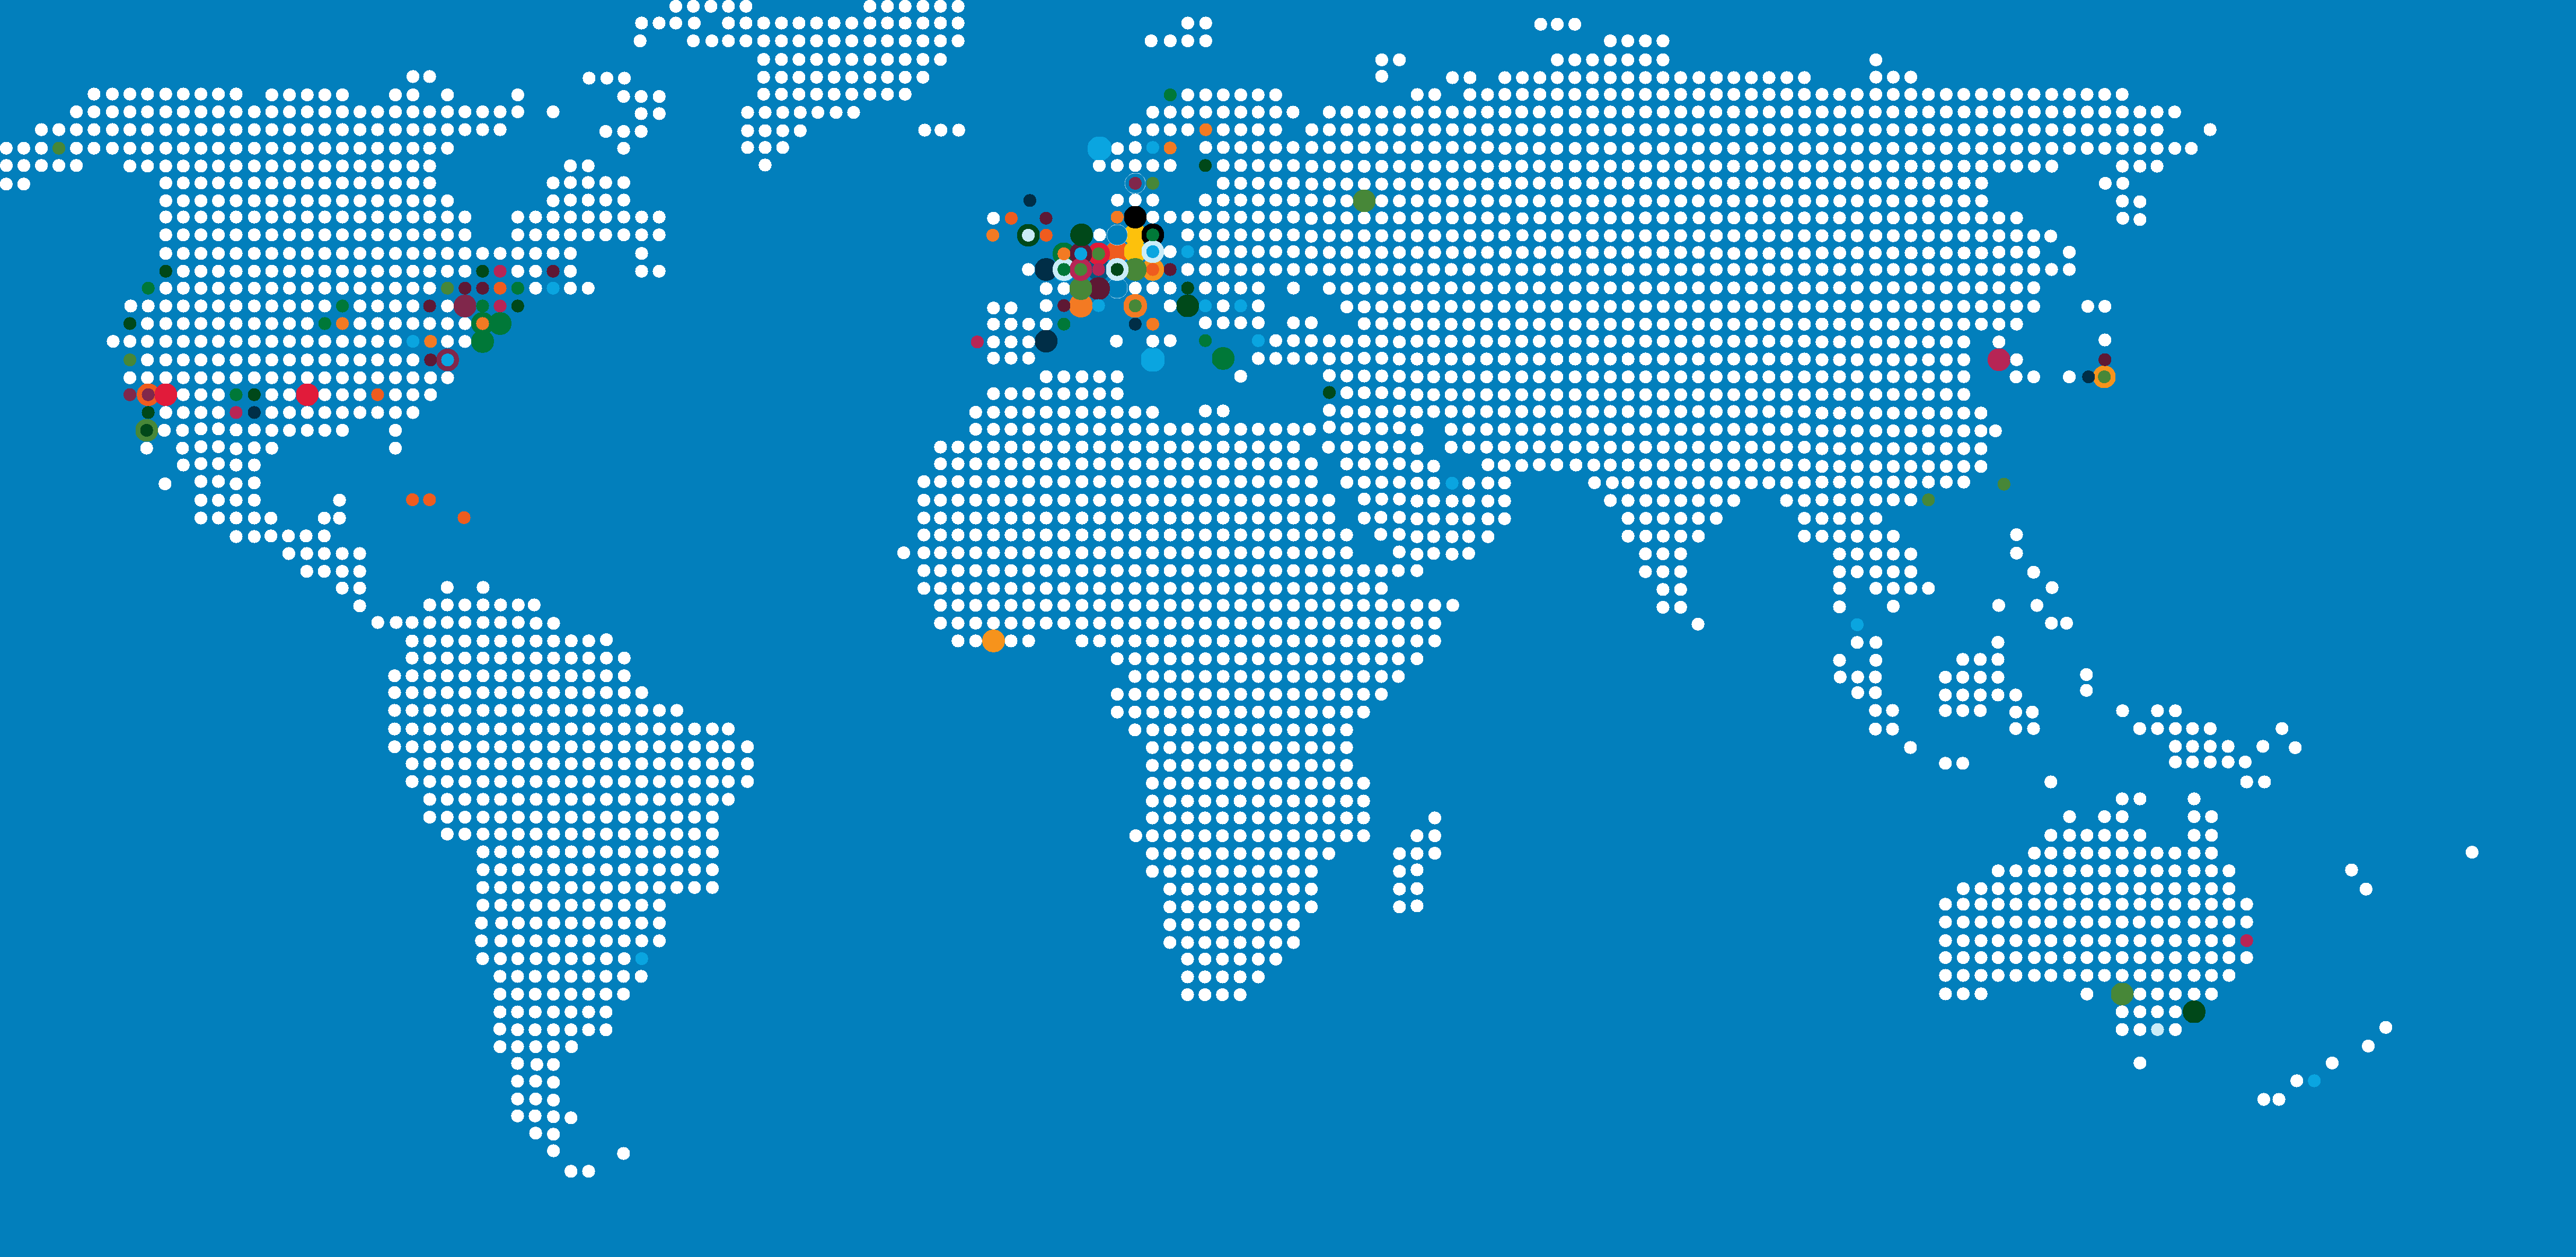
\includegraphics[height=.5\textwidth]{WORLDMAPDOTSdots.png}
}

\section{Language Science Press}
\frame{
\frametitle{Language Science Press}

\begin{itemize}
    \item 45 veröffentlichte Bücher, 305 Interessensbekundungen
    \item  914 \textit{public supporters} + 305 ``anonyme Unterstützer''
    \item Plan ab 2018: 30 Bücher pro Jahr
    \item bis zu >20.000 Downloads pro Buch
  \end{itemize}
     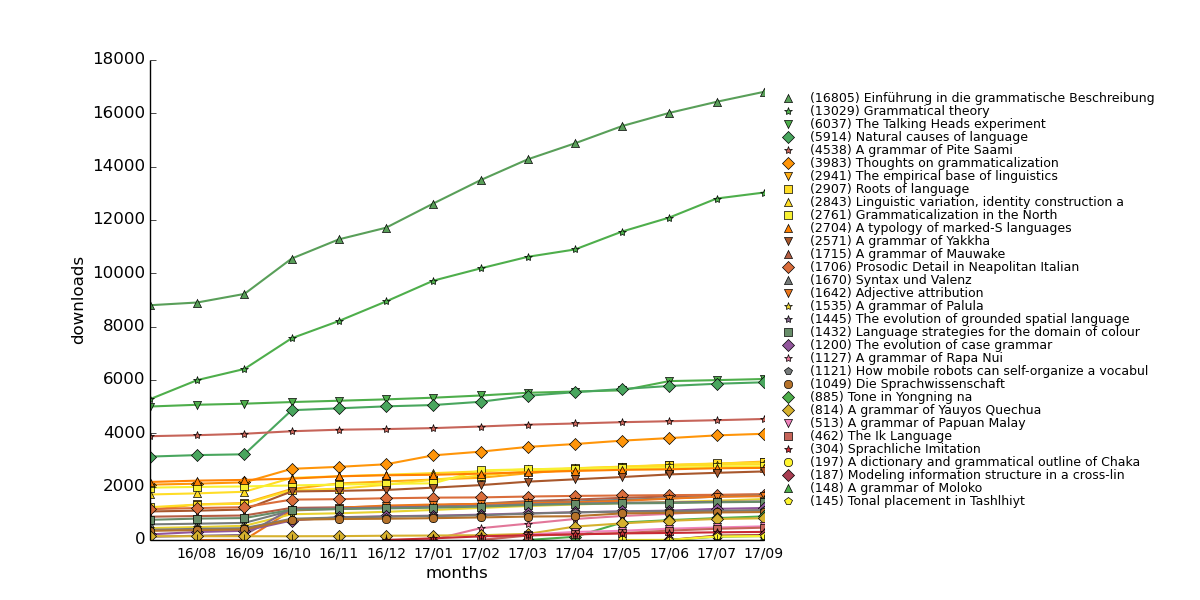
\includegraphics[height=.8\textheight]{./cumulativeallmonograph.png}
}

\frame{
\frametitle{Afrikanistische Bücher bei\newline Language Science Press}
\hfill
\includegraphics[width=2.2cm]{payne}
\hfill
\includegraphics[width=2.2cm]{torrence}
\hfill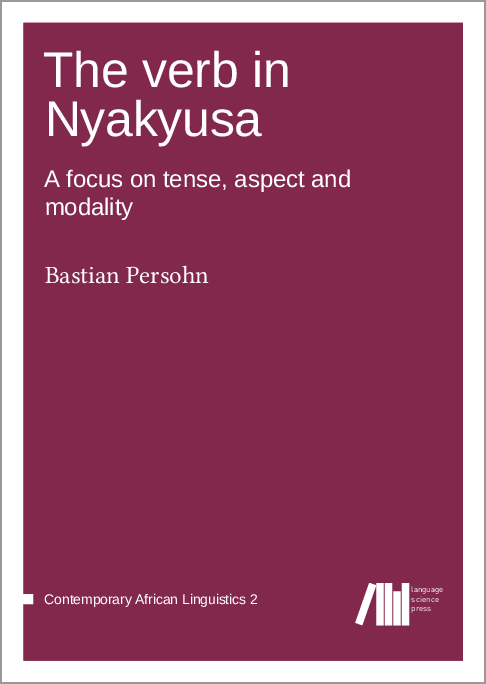
\includegraphics[width=2.2cm]{Persohn} 
\hfill
\includegraphics[width=2.2cm]{schrock}
\hfill\\                   %  .2
\hfill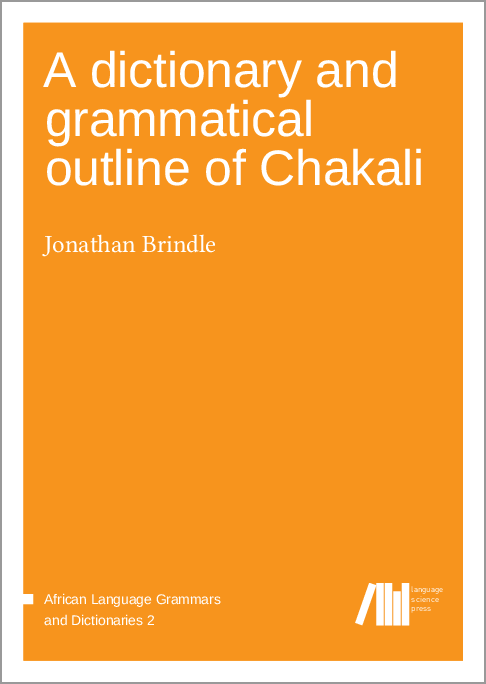
\includegraphics[width=2.2cm]{brindle}
\hfill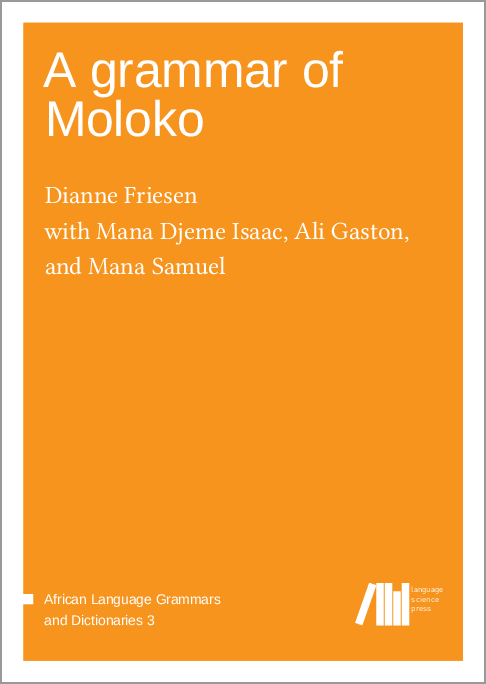
\includegraphics[width=2.2cm]{Friesen}
\hfill
\includegraphics[width=2.2cm]{roettger}
\hfill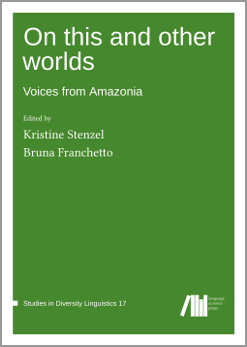
\includegraphics[width=2.2cm]{stenzel}
}

\section{Problemstellung}
\frame{
\frametitle{Ziele von Open Access}
\begin{enumerate}
 \item allgemein zugänglich
 \item billiger 
 \item demokratischer 
\end{enumerate}
}

\frame{
\frametitle{Problemstellung}
\begin{itemize}
 \item Welche Art von OA in den Buchwissenschaften?
 \begin{itemize}
  \item Grüner Weg: allgemein als nicht praktikabel angesehen
  \item Goldener Weg: 	Autorengebühren im fünfstelligen Bereich
  \begin{itemize}
   \item 10.000 EUR (de Gruyter); 18.500 EUR (Brill). 
   \item (vgl. Buchpreis 100 EUR, Auflage 200 = Umsatz 20.000 EUR)
  \end{itemize}
  \item Diamant/Platin-Weg
  \begin{itemize}
   \item Open Library of Humanities; Language Science Press
  \end{itemize}
   \item Community-based publishing
 \end{itemize}
\end{itemize}
}

\section{Marke}  
\frame{
\frametitle{Exkurs: Reclaim the brands!}
\begin{itemize}
 \item Marke = Prestige = bessere Jobchancen = höheres Lebenseinkommen
 \item Monetarisierung der Marken durch Verlage 
 \begin{itemize}
  \item Wertversprechen des höheren Lebenseinkommens
  \item Kosten des Erhalts der Marke sehr gering durch Self-Selection der Einreichenden
 \end{itemize}
 \item Schritte zur Lösung des Geldabflusses aus der Wissenschaft:
 \begin{itemize}
  \item Investition in den Aufbau neuer Marken
  \item \textbf{Absicherung der neuen Marken gegen Übernahmen}
  \begin{itemize}
   \item Negativbeispiele: SSRN, LivingReviews
  \end{itemize}
  \item Markenhoheit bei der Community
 \end{itemize}
\end{itemize}
}

\section{Community}  
\frame{
\frametitle{Was bedeutet \textit{community-based publishing?}}
\begin{itemize}
 \item Marke gehört der Community 
 \item Einbindung der Community
 \begin{itemize}
  \item Advisory Board 
  \item Schriftenreihen 
  \item (Open) Peer Review 
  \item Community Proofreading 
  \item Community Typesetting 
  \item Community Illustration 
  \item Gamification 
 \end{itemize}
 \item Hohe Loyalität
 \item Hohe Durchdringung: bisher 120 verschiedene Community Proofreader
 \item Partizipationsmöglichkeiten auf allen Qualifikationsstufen
  \begin{itemize}
   \item Studenten, Doktoranden, Postdocs, Professoren
  \end{itemize}
\end{itemize}
}
  
\frame{ 
\frametitle{Community: \mbox{Open Review}}
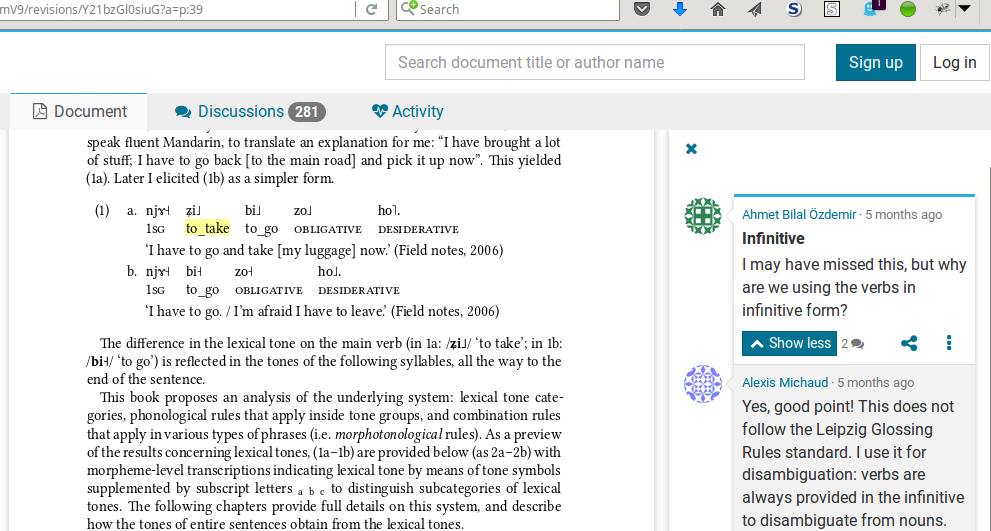
\includegraphics[width=\textwidth]{openreview.png}
}

\frame{ 
\frametitle{Community: \mbox{Community Proofreading}}
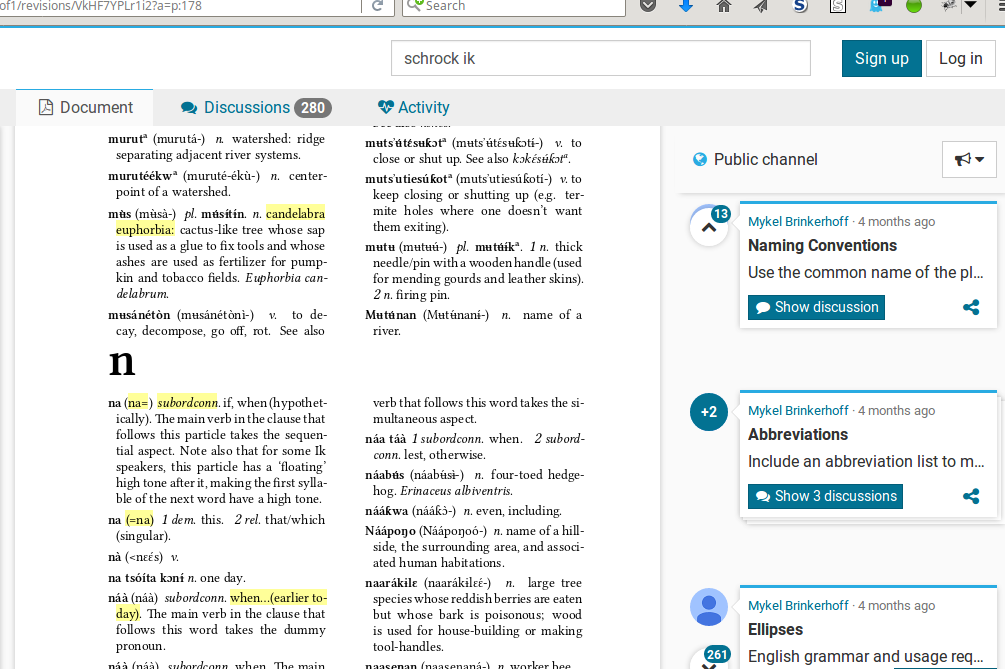
\includegraphics[width=\textwidth]{communityproofreading.png}
}

\frame{ 
\frametitle{Community: \mbox{Hall of Fame}}
\centering
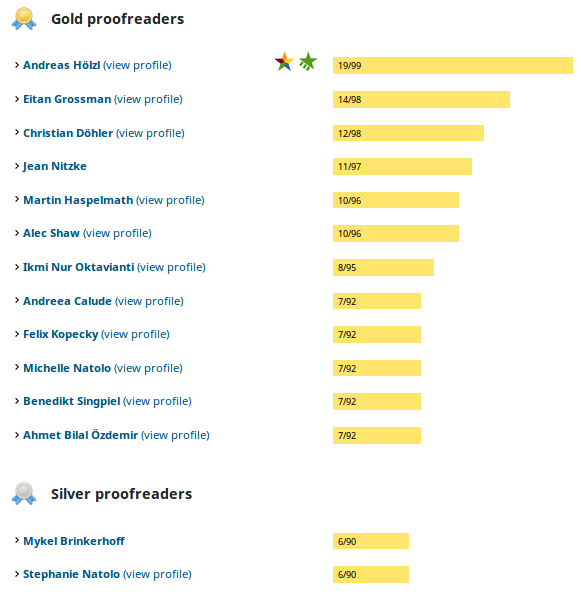
\includegraphics[height=1.2\textheight]{halloffame.png}
}

\section{Offenheit}

\frame{
\frametitle{Offenheit}
%   \includegraphics[height=.2\textheight]{./path/to/graphicsfile}
  \begin{itemize}
    \item  Nur Open-Source-Software, nur CC-BY, transparente Kalkulationen
  \end{itemize}
  
  
\includegraphics[width=3cm]{omp.png} 
  
\includegraphics[width=3.5cm]{github.png} 
  
\includegraphics[width=4cm]{paperhive.png}
  
  
\includegraphics[width=3cm]{overleaf.png}
  
\includegraphics[width=3cm]{ctan.png}
  
\includegraphics[width=3cm]{oapen.png}
  
\includegraphics[width=3cm]{doab.png}
}

    
\frame{
\frametitle{Offenheit: Nachnutzung}
\hspace*{-1cm}
\centering

\includegraphics[height=\textheight]{codingdavinci}
}

\frame{
\frametitle{Offenheit: Nachnutzung}
\begin{itemize}
 \item iPhone-App Languini
\end{itemize}
\centering
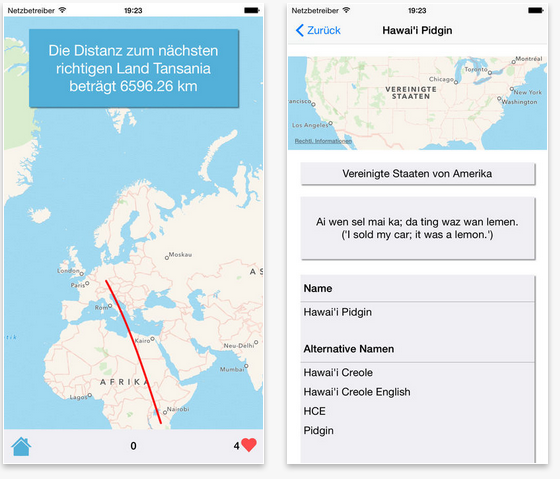
\includegraphics[height=\textheight]{languini}
}


\section{Kosten}

\frame{
\frametitle{Kosten Bottom-Up}
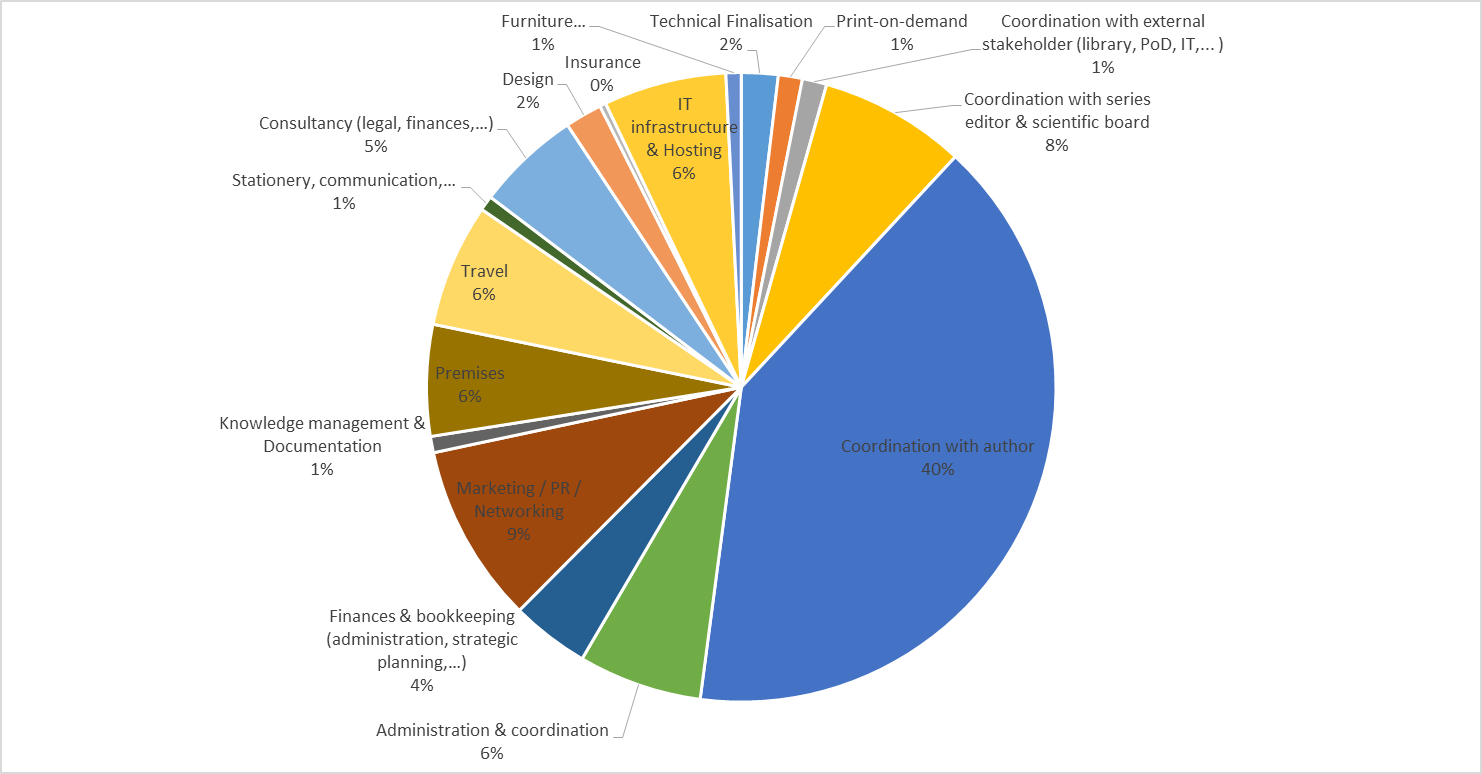
\includegraphics[height=\textheight]{Kuchen.png}
}


\frame{
\frametitle{Kosten Bottom-up}
\hspace*{-.5cm}
\centering
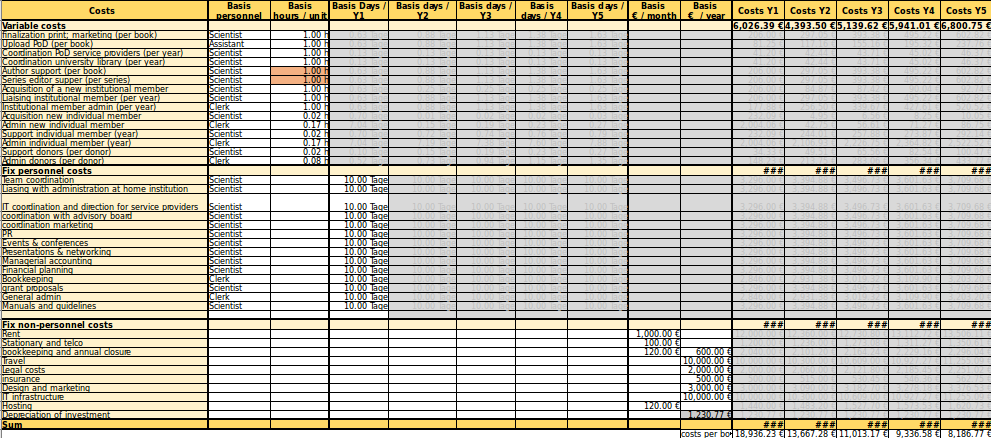
\includegraphics[width=1.1\textwidth]{calculation.png}
\pause
\begin{itemize}
 \item projizierte kalkulatorische Kosten für ein Buch in Jahr 5: 8.186,77 EUR
\end{itemize}
}


\frame{
\frametitle{Kosten: Top-Down}
\begin{itemize}
 \item Förderung DFG 2014-2016: 587.000€
 \item 20 Bücher im Förderungszeitraum veröffentlicht
 \item Kosten pro Buch umgelegt: 29.350€
\end{itemize}
\pause
\begin{itemize}
 \item Laufende Kosten HU im Jahr 2017: \textasciitilde 100.000 EUR 
 \item Stand heute: 22 Bücher im Jahr 2017 veröffentlicht
 \begin{itemize}
  \item bis Ende Dezember voraussichtlich 30 Bücher
 \end{itemize}
 \item Kosten pro Buch umgelegt: 3.333 EUR
\end{itemize}

}
  
\section{Finanzierung}
\frame{
\frametitle{Einnahmearten}
\parbox{.8\textwidth}{
\begin{enumerate}
 \item Spenden \hfill \uncover<2->{2.000 EUR}
 \item Mitgliedschaften\hfill\uncover<3->{100 EUR}
 \item Autorengebühren\hfill\uncover<4->{0 EUR}
 \item Printmarge\hfill \uncover<5->{2.400 EUR}
 \item Institutionelle Mitgliedschaften 
\end{enumerate}
\uncover<7->{~}
}
}

\frame{
\frametitle{Institutionelle Unterstützer}

\begin{itemize}
 \item 100 Forschungseinrichtungen weltweit geben je 1000 EUR/Jahr
 \item Davon werden 30 Bücher pro Jahr als OA produziert
 \begin{itemize}
  \item =33,33 EUR/Buch per Einrichtung
 \end{itemize}
\item Stand heute: 58/100 Unterstützer	
\end{itemize}


\includegraphics[width=\textwidth]{supportinginstitutions.png}
}


 
%\setcounter{framenumber}{\thelastpagemainpart}
\end{document}